\begin{titlepage}
    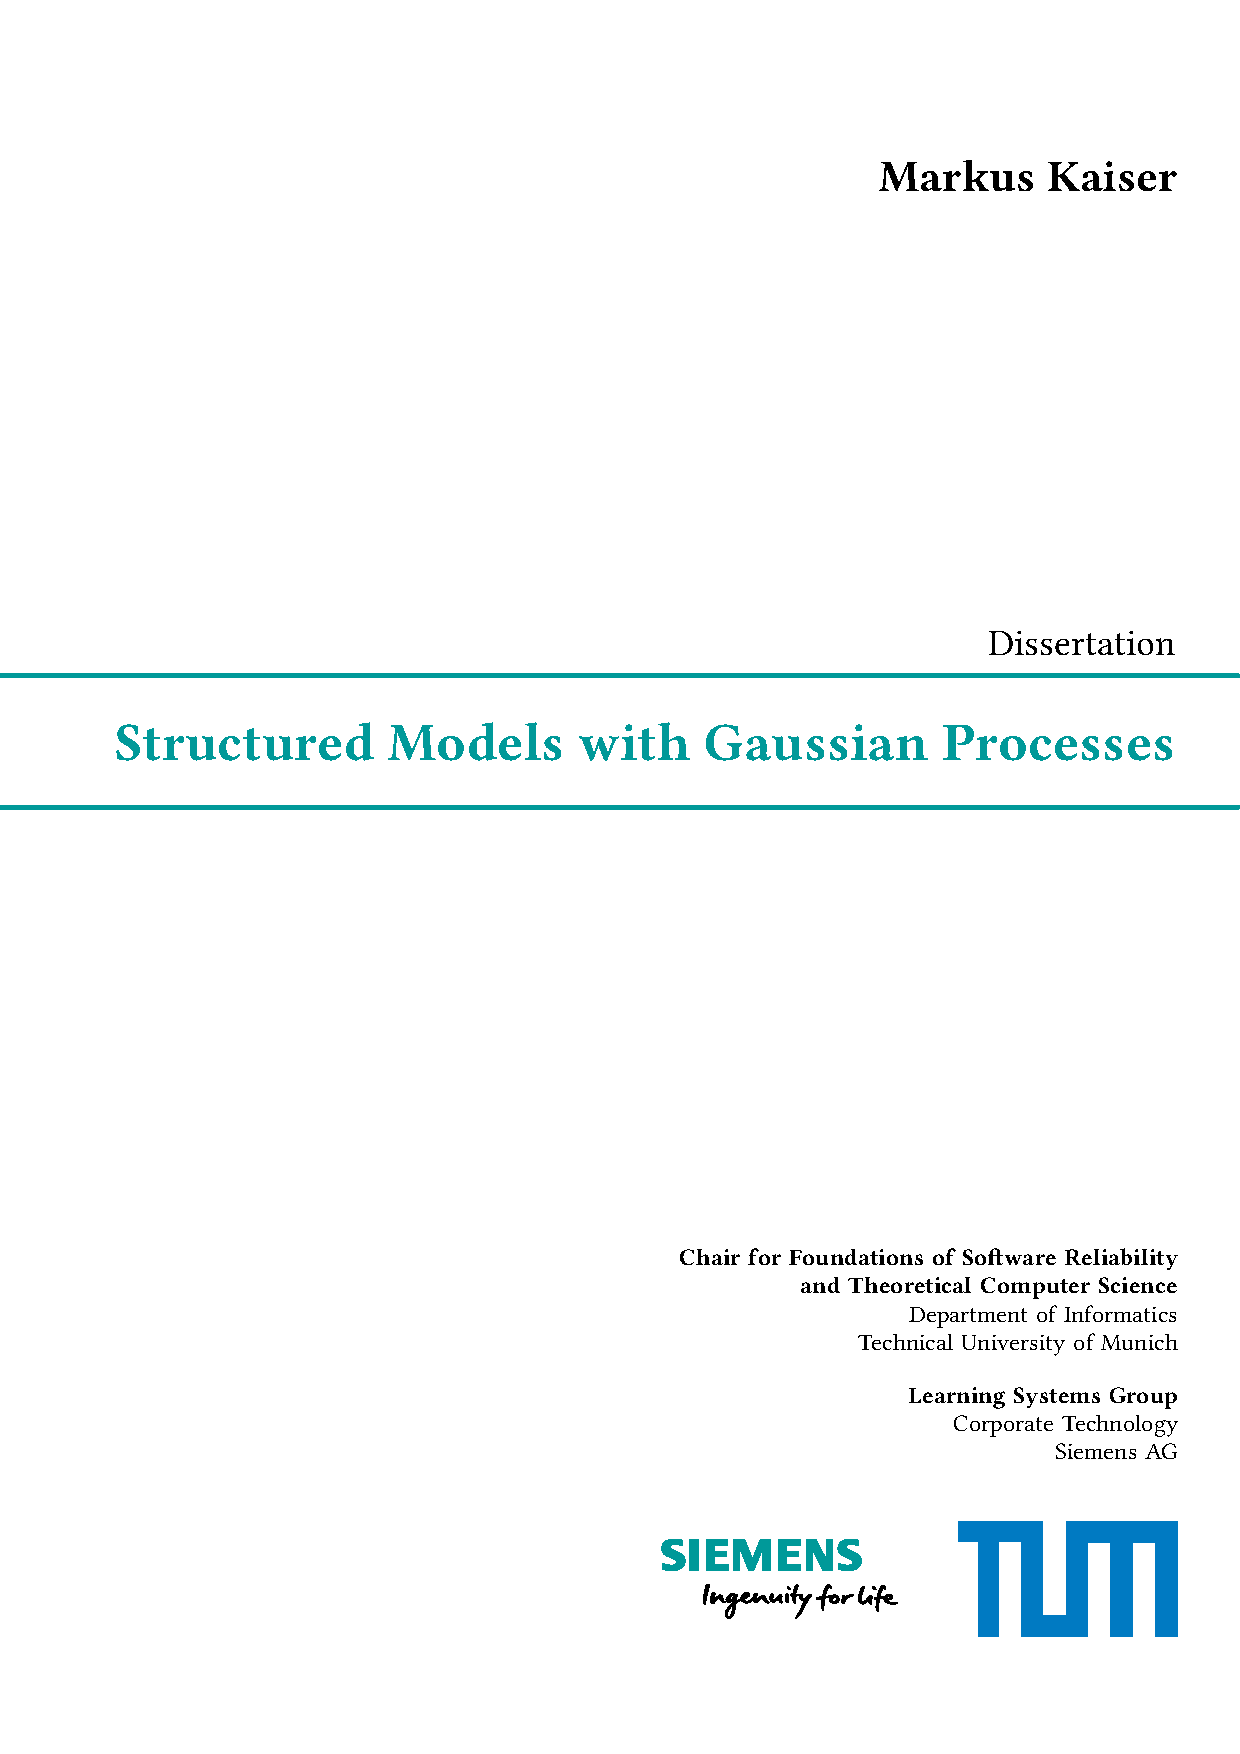
\includepdf{figures/title_page}
\end{titlepage}

\begin{titlepage}
    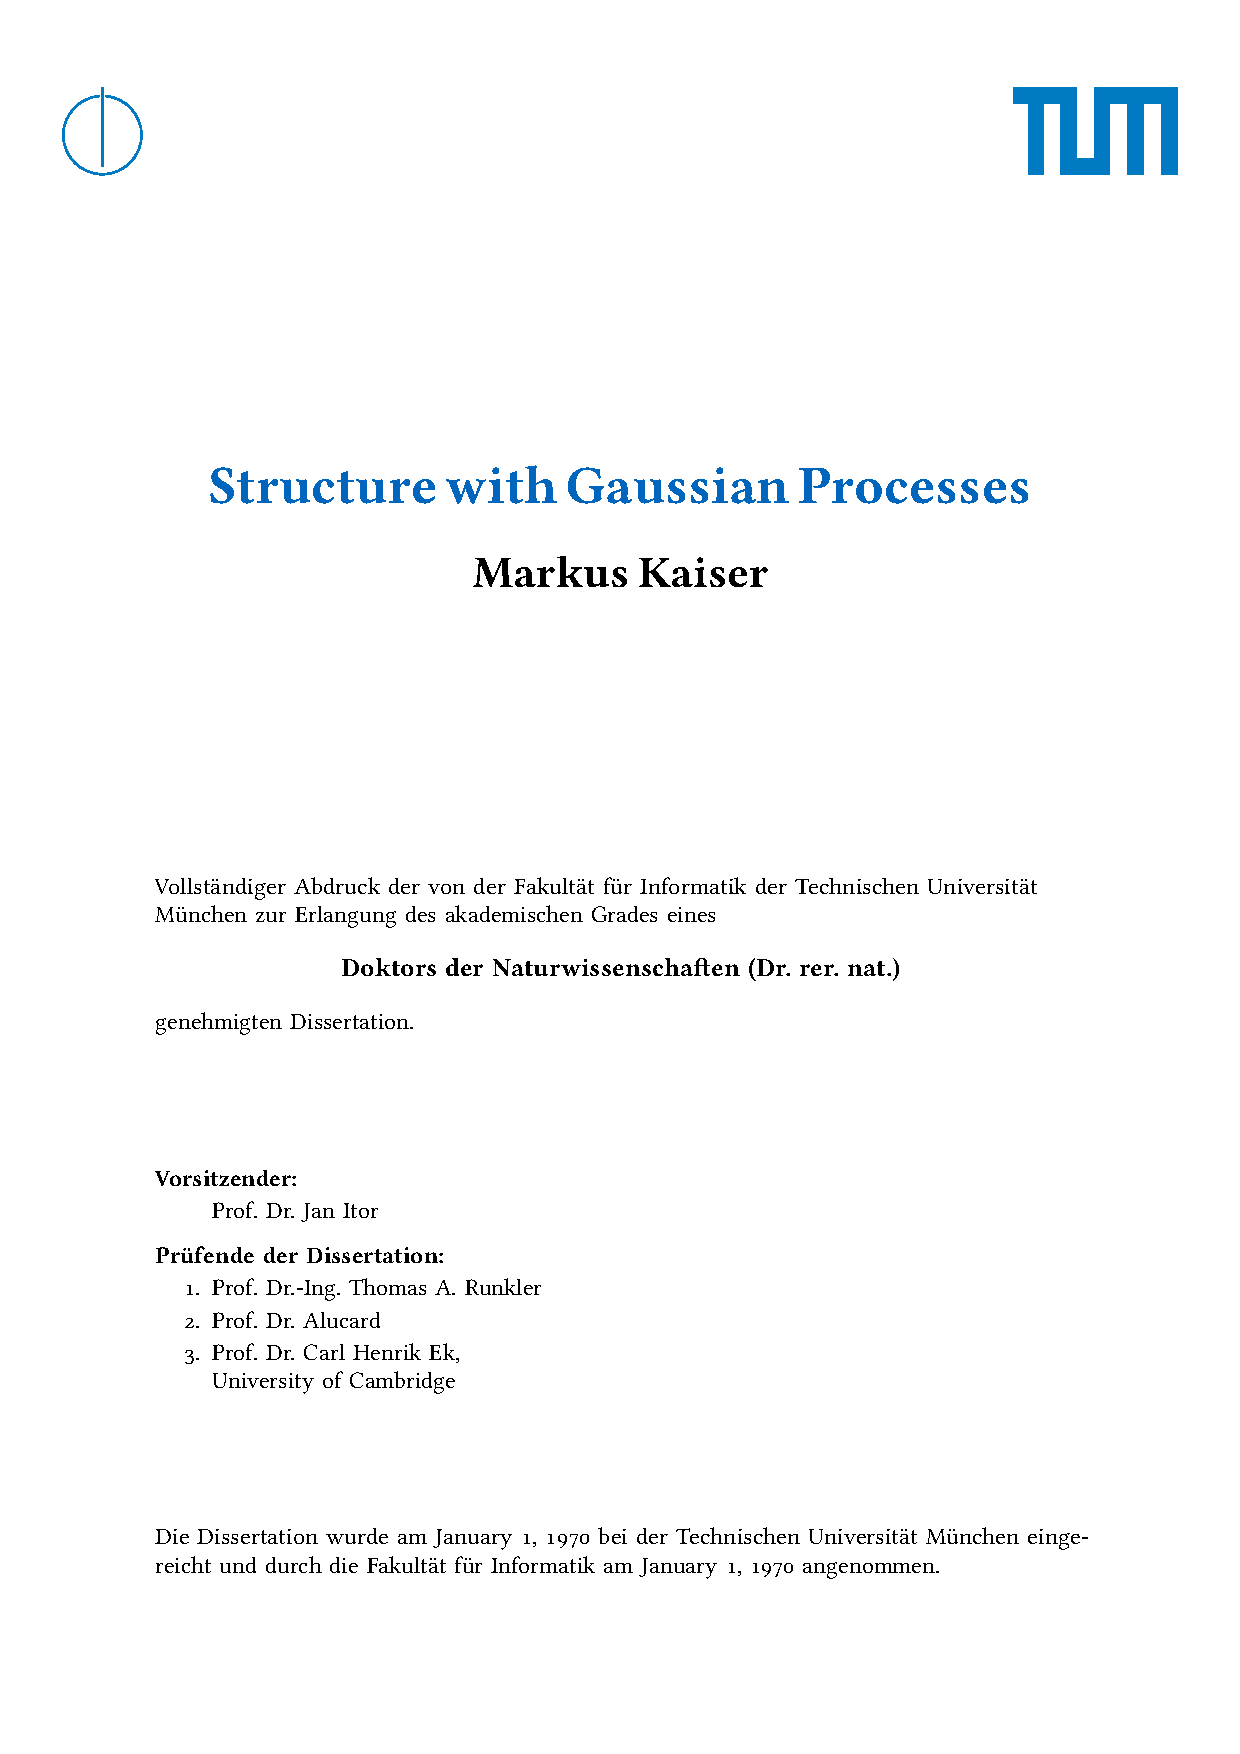
\includepdf{figures/title_page_tum}
\end{titlepage}

\begin{Abstract}{ngerman}
    \todoi{German abstract}
\end{Abstract}

\begin{Abstract}{english}
    Machine learning methods have seen great success recently in a wide range of digital domains such as speech recognition, computer vision or video games.
    However, bridging the gap to applications in the physical world has proved challenging as they introduce a new set of requirements.
    Machine learning systems must make efficient use of expert knowledge, handle low data regimes, and quantify uncertainties.
    This thesis studies how structured probabilistic models allow us to cope with these requirements.
    Structured models combine black-box and white-box modeling approaches to formalize expert knowledge while still being able to gain new insights from data.
    While in white-box models experts design components to describe a generative process in great detail, black-box models rely on general function approximators and trust that structure can be extracted given enough data.
    In structured models, we make use of available expert knowledge but accept that there are parts of the system we do not understand and model them using black-box components.
    Imposing structure allows us to characterize desired solutions and formulate what we want to learn from data.

    In this work, we study how to formulate Bayesian structural models using methods from Bayesian nonparametrics.
    We interpret recent advances in inference schemes for deep Gaussian processes in the context of structural models and formulate informative hierarchical priors.
    We discuss two approaches to adding structure based on mathematical formalization and expert-understanding of an underlying physical process.
    Using real-world industrial applications such as the detection of faulty sensors and the prediction of power generation in a wind-farm as examples, we show how structural priors lead to models with rich internal structure and physically plausible results.

    In situations where internal structure or generalization behavior come into focus, model selection using marginal likelihoods can be insufficient to identify desirable models.
    We consider how to formalize the subjectiveness in model selection through the task a model will be used to solve.
    We show that in a reinforcement learning problem, semantic models outperform other models with similar performance metrics and allow experts to influence agent behavior.
    We finally discuss why models with suboptimal marginal likelihoods can perform well in hierarchical systems and consider how to formulate Bayesian inference problems that take downstream tasks into account.
\end{Abstract}

\begin{Acknowledgements}
    I want to thank my supervisor Prof.~Dr.~Thomas A.~Runkler for his guidance and support.
    Thomas has always encouraged me to explore my ideas while offering invaluable advice and making sure I do not lose focus.
    I am very grateful to my co-supervisor Prof.~Dr.~Carl Henrik Ek for his enthusiasm and mentorship.
    He is an inspiring teacher and shows me what is important in academia.
    Thank you for welcoming me to your research group, making Bristol a second home for me, and the countless discussions about the big picture and the small details.
    I also want to thank my advisor Dr.~Clemens Otte for his valuable input and his exceptional ability to combine research and applications.
    I could not have asked for better supervision or a more encouraging research environment during my studies.

    I am thankful to everyone at Siemens and the Learning Systems group, especially Volkmar Sterzing for giving us PhD candidates the freedom to pursue our interests and enabling us to work on exciting industrial applications.
    I am grateful to Steffen Udluft and Hans Georg Zimmermann for always taking the time to discuss new ideas and for broadening my horizon as well as my fellow PhD candidates Stefan Depeweg, Daniel Hein and Phillip Swazinna for many discussions, whiteboard-drawings and meetings at the Biergarten.
    Thanks to Marion Eigner for her refreshing perspective and friendship.

    I feel lucky to be part of a motivating and unique group in Bristol and Bath.
    Thank you to Prof.~Dr.~Neill Campbell for your passion for good research and for your help in pursuing worthwhile ideas.
    I want to thank Erik Bodin, Ieva Kazlauskaite and Ivan Ustyuzhaniov for many thoughtful discussions and collaborations.

    A big thank you to my siblings Matthias and Andrea for your support and encouragement.
    I sincerely thank my parents, Pia and Robert Kaiser, for enabling and inspiring us to follow our dreams and for your unconditional support.
    Above all I want to thank Hannah for her patience and understanding while being in COVID-19 lockdown with a person writing their thesis.
    Thank you for all the lunches, the much-needed distractions, the happiness, and your love.
\end{Acknowledgements}

\listoftodos
\todototoc

\tableofcontents
